\section{Project Plan}

\begin{frame}
	{Slides}

	\begin{itemize}
		\item
			Download the slides for local reference
		\item
			\url{https://cm.e-ale.org/2019/SCaLE17x/iio/iioinput-user-SLIDES.pdf}
	\end{itemize}
\end{frame}

\begin{frame}
	{What To Do?}

	\begin{itemize}
		\item
			Check out that cool thumbwheel on the BaconBits MiniCape.
		\item
			Let's do something with it!
		\item
			We'll learn how to read the position of the thumbwheel.
		\item
			With that data, we have the foundation for a userspace single axis joystick driver.
	\end{itemize}

	     \begin{figure}[H]
		     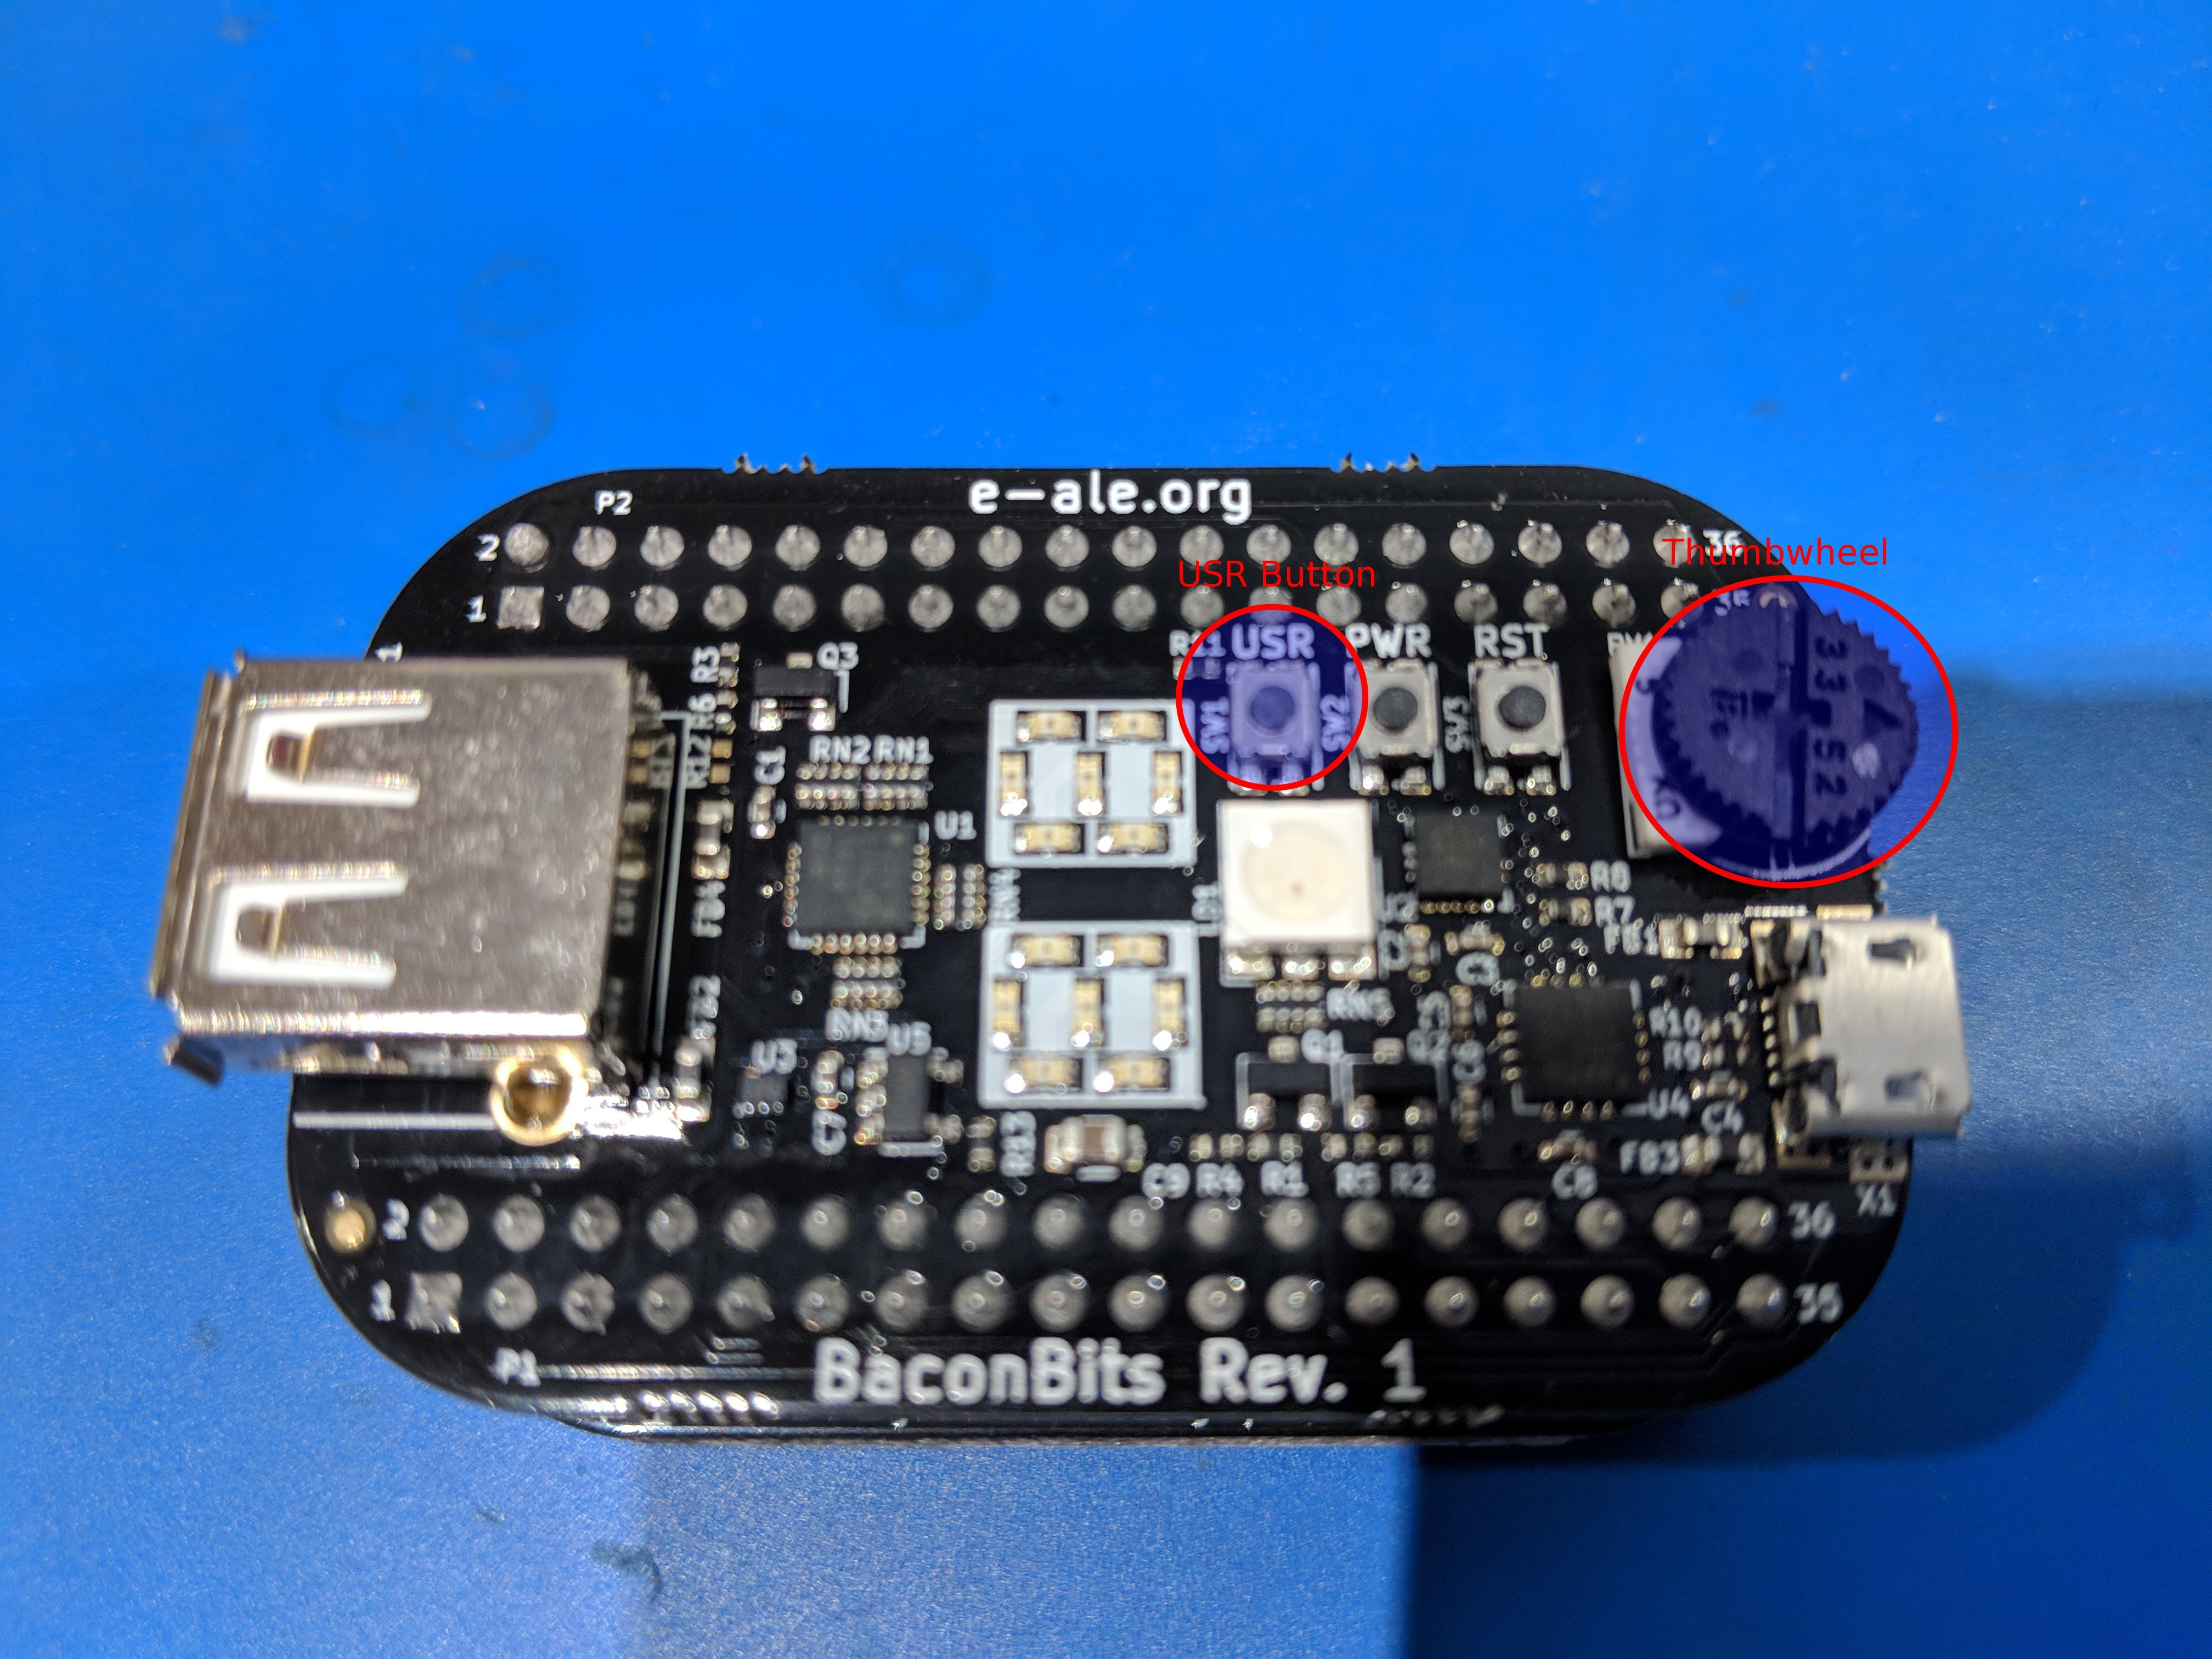
\includegraphics[width=3in]{IMAGES/baconbits-annotated}
				       \caption{BaconBits MiniCape}
	     \end{figure}
\end{frame}


\begin{frame}
	{Exact Steps}
	\begin{itemize}
		\item
			Understand how the thumbwheel is interfaced in hardware
		\item
			Understand IIO and its purpose in the universe
		\item
			Learn how IIO exposes the thumbwheel's ADC to userspace
		\item
			Learn how to use libiio for userspace IIO interaction
		\item
			Write a thumbwheel-based userspace joystick driver and test it
	\end{itemize}
\end{frame}
